\documentclass[11pt]{article}

\usepackage[T1]{fontenc}
\usepackage[utf8]{inputenc}
\usepackage{lmodern}
\usepackage{microtype}
\usepackage[margin=1.15in]{geometry}
\usepackage{graphicx}
\usepackage{booktabs}
\usepackage{amsmath,amssymb}
\usepackage{xcolor}
\definecolor{slate}{HTML}{2A4A6A}
\definecolor{rulecol}{HTML}{C3C2B7}
\definecolor{ink}{HTML}{1A1A19}
\usepackage[colorlinks=true,linkcolor=slate,urlcolor=slate,citecolor=slate]{hyperref}
\usepackage{caption}
\captionsetup{font=small,labelfont=bf,labelsep=period,width=0.95\linewidth}
\makeatletter
\renewcommand\section{\@startsection{section}{1}{\z@}{1.4em}{0.5em}{\normalfont\large\bfseries\color{slate}}}
\renewcommand\subsection{\@startsection{subsection}{2}{\z@}{1em}{0.4em}{\normalfont\normalsize\bfseries\color{ink}}}
\makeatother

\newcommand{\rs}{\text{Rs}\,}

\title{\vspace{-3.5em}\textbf{\LARGE Anatomy of a False Edge}\\[0.35em]
\normalsize\normalfont A Falsification of a Microstructure Market-Making Strategy\\ on NSE Equity Futures}
\author{Krishhiv Mehra}
\date{July 2026}

\begin{document}
\maketitle
\thispagestyle{empty}

\begin{abstract}
\noindent This report documents a self-directed research project that built a live
paper-trading system for a microstructure market-making strategy on National Stock
Exchange (NSE) equity futures, and then falsified it. Under the simulator's optimistic
touch-fill model the strategy appeared strongly profitable. A markout and mid-to-mid
decomposition, computed directly from the stored order book, shows that the entire
reported profit was an artifact of assumed bid-ask spread capture: priced at the mid,
the strategy lost $\rs 10.14$ lakh and its win rate collapsed from 77\% to 12.6\%,
exposing a \emph{negative} directional edge. Break-even requires retaining at least
81\% of the theoretical spread, a level a non-colocated retail participant cannot reach
given back-of-queue priority, roughly 15\,ms latency, and a securities transaction tax
that dominates round-trip cost. Overfitting-aware evaluation (Deflated Sharpe Ratio,
Probability of Backtest Overfitting) promoted no variant. The project was halted at this
documented verdict and its design pivoted toward taker-side, model-based strategies at
horizons where latency does not decide the outcome. No real capital was deployed.
\end{abstract}

\vspace{0.5em}
{\small\tableofcontents}
\thispagestyle{empty}
\newpage

\section{Introduction and motivation}

This is a falsification study. It documents how a systematic trading strategy that looks
profitable in simulation can be an artifact of its fill model, how to detect that before
committing capital, and why the resulting verdict was specific to the trading seat rather
than to the idea. The deliverable is the method and the decision, not a strategy that works.

The strategy is a passive market maker driven by a single signal, the microprice deviation
from the level-one order book,
\[
\text{microprice} = \frac{\text{bid}_{\text{px}}\cdot\text{ask}_{\text{qty}} + \text{ask}_{\text{px}}\cdot\text{bid}_{\text{qty}}}{\text{bid}_{\text{qty}}+\text{ask}_{\text{qty}}},
\qquad
\text{deviation} = \text{microprice} - \text{mid},
\]
an imbalance-weighted fair value that leans toward the heavier side of the book \cite{stoikov}.
The strategy posts a passive limit order at the bid or ask when the deviation exceeds a floor
and an economic edge gate is satisfied (the captured half-spread must cover the per-share
round-trip fee), then exits passively at the opposite side, with taker fallbacks on a hard
stop and a hold-time limit. The intent is to earn the spread rather than pay it.

\section{Data and experimental design}

A collector on a Mumbai cloud VPS archives the full NSE 20-level tick-by-tick order book for
a liquid futures universe, stored as date-partitioned Parquet. This order book is the raw
material for every result below.

Strategy variants were compared \emph{live and head-to-head} rather than by backtest, for a
specific reason: a compacted-data replay of the strategy missed a live trading day by
$\rs 11$k, which localised the unreliability to the fill model, the one component a backtest
cannot get right. The system therefore ran a multi-arm harness: seven ``arms'' (a control
plus challengers varying stop width, universe, selectivity, and exit logic) fed by one shared
depth connection, each with isolated brokers, an independent risk governor, and namespaced
logs, so arms never contaminate one another. Champion-versus-challenger on identical live data
is the only trustworthy way to compare variants when the simulator itself is suspect. The
analysis below covers twelve clean trading days.

\section{The apparent result, and the first red flag}

On the simulator's touch-fill model (a passive order fills the instant price touches its
level) the strategy looked strongly profitable, with a win rate near 77\%. The first sign
that this was not what it seemed was a unit check: the strategy captured roughly $4.5$ basis
points of gross profit per trade, while the half-spread on these instruments is only about
$0.2$ to $0.4$ basis points. A market maker's edge \emph{is} the spread; capturing fifteen to
twenty-five times the spread means the profit is coming from \emph{directional} price moves,
not from providing liquidity, and directional capture is precisely where an optimistic fill
model is least trustworthy.

\section{Method: the mid-to-mid decomposition}

Two quantities, both computed straight from the stored order book and therefore independent of
the fill model, separate assumed spread capture from realised price movement.

\paragraph{Markout.} For a fill at price $p$ in direction $d\in\{+1,-1\}$,
\[
\text{markout}(h) = d\,\big(\text{mid}(t_{\text{fill}}+h) - p\big).
\]
At $h=0$ this is the captured half-spread (a passive fill sits inside the mid); as $h$ grows it
reveals any adverse drift after the fill.

\paragraph{Mid-to-mid profit and loss.} Re-pricing \emph{both} legs of a round trip at the mid,
\[
\text{P\&L}_{\text{mid}} = d\,\big(\text{mid}_{\text{exit}} - \text{mid}_{\text{entry}}\big)\cdot\text{qty} - \text{fee},
\]
removes all spread capture and leaves the pure directional result. The two views satisfy the
identity
\[
\text{P\&L}_{\text{sim}} = \text{P\&L}_{\text{mid}} + \text{(assumed spread capture)},
\]
so decomposing the simulated profit isolates exactly how much of it was the spread the model
handed itself for free.

\section{Results}

The decomposition is unambiguous (Figure~\ref{fig:decomp}). Of the simulated
$+\rs 2.38$ lakh, \emph{all} of it, and $\rs 10.14$ lakh more, is assumed spread capture; the
directional component priced at the mid is $-\rs 10.14$ lakh. The win rate falls from 77\% on
the simulator to 12.6\% at the mid. The strategy has no directional edge; it is a pure spread
harvester whose ``wins'' are the spread assumption.

\begin{figure}[t]
\centering
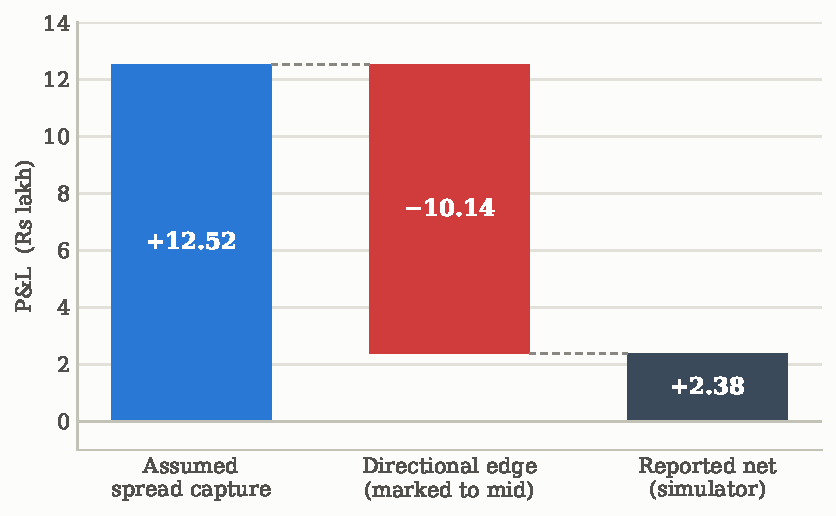
\includegraphics[width=0.82\linewidth]{figures/decomposition.pdf}
\caption{The simulated profit decomposed. Marking both legs to the mid removes the assumed
bid-ask capture and reveals a large negative directional result. The reported net is a thin,
fragile residual on top of a spread assumption five times its size.}
\label{fig:decomp}
\end{figure}

The pattern is universal across the universe (Figure~\ref{fig:instr}), not driven by one name.
The apparent top earner, AXISBANK at $+\rs 1.32$ lakh, is $-\rs 3.24$ lakh once priced at the
mid; every instrument flips negative.

\begin{figure}[t]
\centering
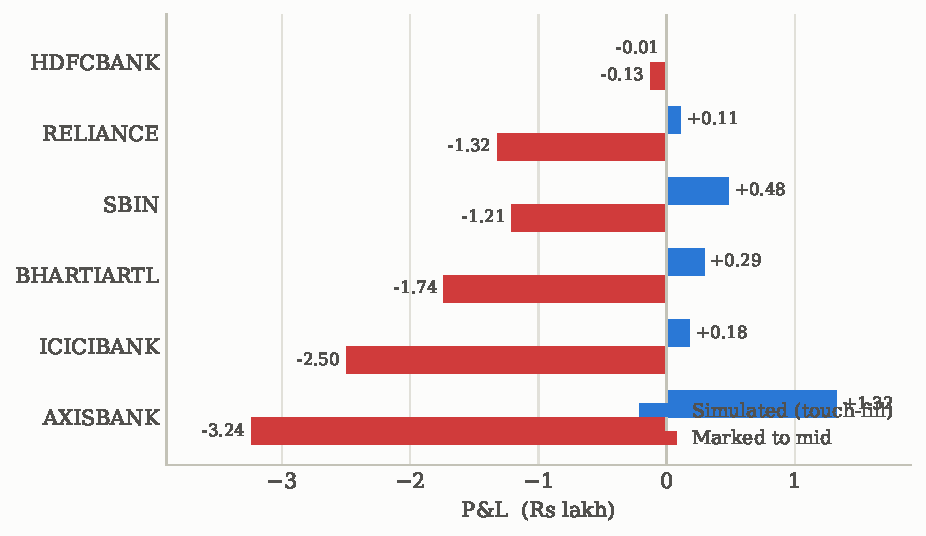
\includegraphics[width=0.82\linewidth]{figures/instruments.pdf}
\caption{Per-instrument profit, simulated versus marked to mid. The spread-capture illusion is
present in every name; the strongest apparent earners are the largest at-mid losses.}
\label{fig:instr}
\end{figure}

The markout curve (Figure~\ref{fig:markout}) sharpens the diagnosis. The entry markout is
positive and roughly flat out to sixty seconds ($\rs 197$ at the fill, $\rs 176$ at
$60$\,s), so the favourable fill is real at the instant of execution and the entry is
\emph{not} catastrophically adversely selected at these horizons. The loss does not accrue at
entry; it accrues between entry and exit, where the mid drifts against the position and only
the spread assumption keeps the trade in the black.

\begin{figure}[t]
\centering
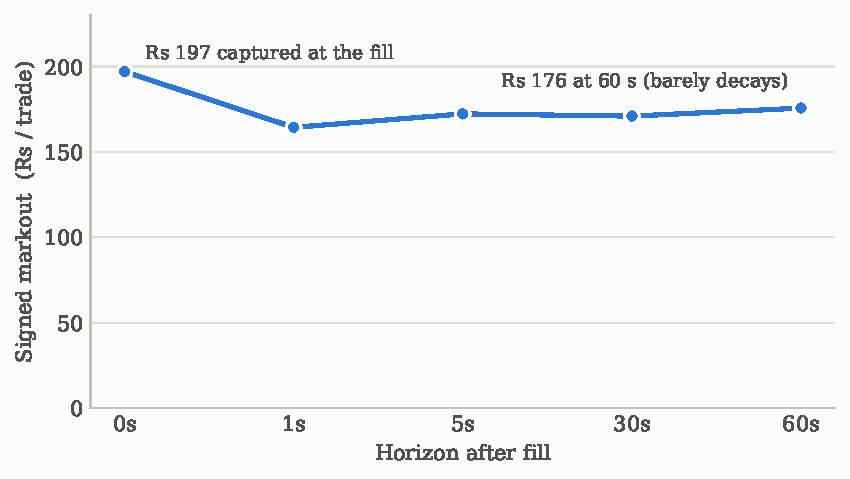
\includegraphics[width=0.80\linewidth]{figures/markout.pdf}
\caption{Signed entry markout by horizon. The half-spread captured at the fill is real and
barely decays, so entry toxicity is not the mechanism; the negative result lives in the
exit-side price drift that the mid-to-mid view exposes.}
\label{fig:markout}
\end{figure}

Finally, the decomposition sets a hard target (Figure~\ref{fig:break}). Writing realistic net
as $\text{P\&L}_{\text{mid}} + f\cdot(\text{spread capture})$ for a retained spread fraction
$f$, break-even occurs at $f^{*}=81\%$. Independently, a queue-aware fill simulation placed
the break-even maker-exit fill rate near 67 to 80\%, corroborating the threshold by a second,
unrelated method.

\begin{figure}[t]
\centering
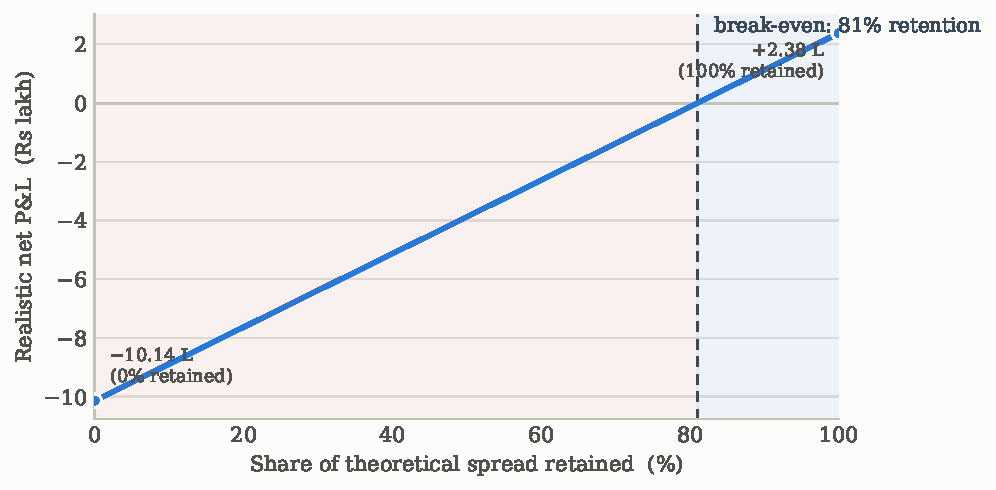
\includegraphics[width=0.80\linewidth]{figures/breakeven.pdf}
\caption{Profitability as a function of how much of the theoretical spread is actually retained.
Break-even needs 81\% retention; realistic execution must land far toward the favourable end of
this line, which is the hard direction to reach, not the easy one.}
\label{fig:break}
\end{figure}

\section{Statistical rigour: subtracting luck}

A multi-arm race makes the best arm look good by chance alone, so no arm was trusted on its raw
numbers. Arms were ranked on cost-realistic, out-of-sample returns using the effective sample
size $n_{\text{eff}}$ (trades are autocorrelated, so the raw count overstates information), the
Probabilistic and Deflated Sharpe Ratios \cite{psr,dsr}, and the Probability of Backtest
Overfitting via combinatorially-symmetric cross-validation \cite{pbo}. The promotion gate was
$\text{DSR}\geq 0.95$ and $\text{PBO}\leq 0.2$.

The best arm reached a Deflated Sharpe of $0.93$, short of the gate, on returns that were
themselves optimistic; the Probability of Backtest Overfitting was near zero, indicating the
\emph{selection} was sound while the \emph{edge} was not. The statistical verdict and the
execution-realism finding agree: there was nothing to promote.

\section{Interpretation: a structural, seat-specific verdict}

The strategy is a pure spread harvester with a negative directional edge, so its survival
depends entirely on spread retention, which is governed by queue position. A retail seat cannot
reach the required 81\%. It sits at the back of a first-in-first-out queue without colocation,
acts at roughly 15\,ms latency, earns no maker rebate on this segment, and pays a securities
transaction tax (STT) that is about two-thirds of round-trip cost and falls on a seconds-hold,
one-tick-spread strategy that cannot out-earn it (Table~\ref{tab:fees}).

\begin{table}[h]
\centering
\caption{Per-instrument cost, one lot. STT scales with the sell-side notional, so the
break-even move per share, not a flat threshold, is the economically meaningful quantity, and
it varies roughly threefold across the universe.}
\label{tab:fees}
\small
\begin{tabular}{lcc}
\toprule
Instrument & Round-trip fee & Break-even move / share \\
\midrule
HDFCBANK  & $\sim\rs 126$ & $\rs 0.23$ \\
RELIANCE  & $\sim\rs 177$ & $\rs 0.35$ \\
ICICIBANK & $\sim\rs 222$ & $\rs 0.32$ \\
\bottomrule
\end{tabular}
\end{table}

The subtle point is \emph{where} the adverse selection lives. It is not mainly in the markout
horizon, which is flat-positive; it is in fill \emph{selection}. From the back of the queue you
miss the benign touches (price taps your level and bounces, the resting orders ahead of you
absorb it, and you do not fill) and you keep the adverse breaks (price trades through, the queue
clears, and you fill an instant before the move continues against you). The touch-fill model
deletes this bias by construction because it fills on every touch; pricing at the mid restores
it. Relatedly, the microprice does predict the next tick, but the colocated participants who set
it act microseconds after the book changes, so at retail latency one trades \emph{after} the
information is already in the price. The signal is real; the seat cannot reach it.

\section{The pivot: seat-first strategy design}

Rather than tune a structurally dead strategy, the design was re-derived from the seat outward:
given no colocation, no exchange membership, no rebates, roughly 15\,ms latency, and small
capital, which edges are even available? The market-making (latency-race) game is closed to that
seat. What remains open is \emph{taker-side, model-based} strategies at horizons where latency
does not decide the outcome: statistical arbitrage and Ornstein-Uhlenbeck mean-reversion,
principal-component residual reversion \cite{avellaneda}, cross-sectional short-horizon reversal
\cite{lomackinlay}, and calendar spreads, each derived from a testable statistical property
(cointegration \cite{englegranger}, factor structure, order-flow impact \cite{cont}) rather than
a tuned chart indicator. A three-year daily and one-minute historical dataset was assembled as
the foundation for that program.

\section{Conclusion}

The market-making strategy has no viable edge for a self-funded retail seat, and its only path
to profitability requires institutional execution infrastructure, colocation, FPGA order
handling, and exchange membership, that is outside a bootstrapped budget. The identified pivot is
a longer research program that would need either risk capital or more runway. Given that, the
disciplined choice was to halt at a clean, documented stopping point rather than deploy capital
into an unvalidated strategy.

The value delivered is the research itself: a method (the markout and mid-to-mid decomposition,
paired with overfitting-aware evaluation) that separates a real edge from a fill-model artifact;
a finding (a strategy that looked profitable was falsified) reached on paper with zero capital at
risk; and the judgment to stop. A false edge is cheapest to discover before it is funded.

\begingroup
\small
\begin{thebibliography}{9}
\bibitem{stoikov} Stoikov, S. (2018). The micro-price: a high-frequency estimator of future prices. \emph{Quantitative Finance}, 18(12).
\bibitem{psr} Bailey, D.~H., and L\'opez de Prado, M. (2012). The Sharpe Ratio Efficient Frontier. \emph{Journal of Risk}, 15(2).
\bibitem{dsr} Bailey, D.~H., and L\'opez de Prado, M. (2014). The Deflated Sharpe Ratio. \emph{Journal of Portfolio Management}, 40(5).
\bibitem{pbo} Bailey, D.~H., Borwein, J.~M., L\'opez de Prado, M., and Zhu, Q.~J. (2017). The Probability of Backtest Overfitting. \emph{Journal of Computational Finance}, 20(4).
\bibitem{cont} Cont, R., Kukanov, A., and Stoikov, S. (2014). The price impact of order book events. \emph{Journal of Financial Econometrics}, 12(1).
\bibitem{avellaneda} Avellaneda, M., and Lee, J.-H. (2010). Statistical arbitrage in the US equities market. \emph{Quantitative Finance}, 10(7).
\bibitem{englegranger} Engle, R.~F., and Granger, C.~W.~J. (1987). Co-integration and error correction. \emph{Econometrica}, 55(2).
\bibitem{lomackinlay} Lo, A.~W., and MacKinlay, A.~C. (1990). When are contrarian profits due to stock market overreaction? \emph{Review of Financial Studies}, 3(2).
\end{thebibliography}
\endgroup

\vfill
{\footnotesize\noindent\textit{All trading described in this report was simulated on live and
historical market data. No orders were sent to a live exchange and no real capital was deployed.}}

\end{document}
